\section{Additional Experimental Results}

% \subsection{Other Attempts}
\subsection{RL with Agentic Step as Action}
To mitigate the high variance inherent in token-level value predictions, we implement a step-wise GAE calculation. We define a step (denoted as $S_i$) as a single conversation turn and assume that all constituent tokens share a uniform learning signal within each step. We define the step-level value $V(S_i)$ using two primary aggregation methods based on constituent token values predictions $\{v_{i,1}, v_{i,2}, \dots, v_{i,n}\}$: 

\begin{itemize}[leftmargin=*,itemsep=0pt,parsep=0.2em,topsep=0.3em,partopsep=0.3em]
\item \textit{Step Average.} The step value is the average of all token value predictions within that step, $V(S_i) = \frac{1}{n} \sum_{j=1}^{n} v_{i,j}$. In this setting, the value model is trained on all tokens. 
\item \textit{Last-Token Prediction.} We define the step value as $V(S_i) = v_{i,n}$, using only the final token of each step, assuming that the final token provides the most accurate value prediction of the step, as it encapsulates the most comprehensive information of the entire unit. During value model training, we apply a loss mask to all intermediate tokens, ensuring that only the last token of each step contributes to the optimization.
\end{itemize}

To provide a more stable learning signal, we implement a step-wise GAE calculation that shifts the advantage estimation from a token-level to a step-level granularity. We derive a single advantage $\hat{A}_i$ for each step based on the step-level TD error $\delta_i = R_i + \gamma V(S_{i+1}) - V(S_i)$. This advantage is then assigned uniformly to all tokens within the corresponding step, effectively smoothing out the local noise prevalent in auto-regressive generation. Furthermore, the length-adaptive GAE mechanism is modified to scale the decay factor $\lambda$ based on the total number of steps rather than the raw token length, where $$\lambda_{\text{policy}} = 1 - \frac{1}{\alpha * \text{step number}}$$

However, as illustrated by the training reward in Figure \ref{fig:reward_curve} and the performance results in Table \ref{tab:stepwise_training}, both step-wise approaches underperform token-wise value training. We attribute this failure to the fact that token-level training provides a finer-grained supervision signal for both the critic and the policy, which is essential for accurately capturing the logical transitions within complex reasoning trajectories.


\begin{figure}[ht]
\centering
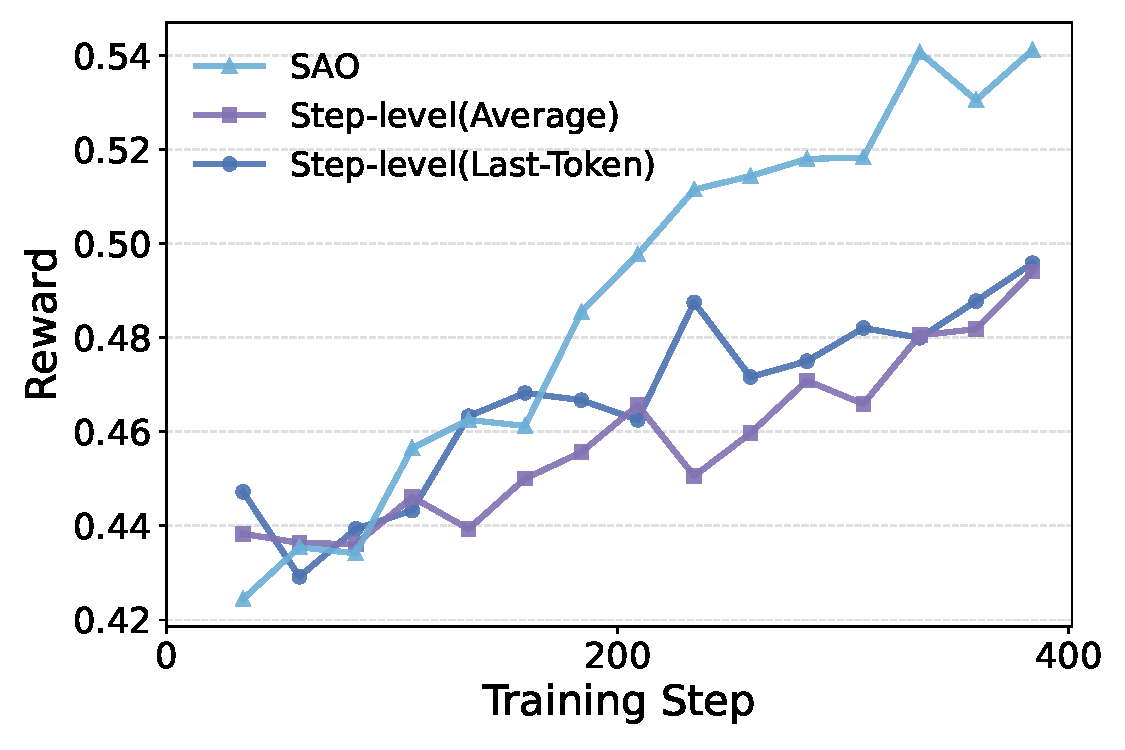
\includegraphics[width=0.45\textwidth]{figures/stepwise_trainingreward.pdf}
\caption{Training reward for token-level \model training and step-level variants, where token-level shows better training rewards.}
\label{fig:reward_curve}
\end{figure}



\begin{table}[htbp]
\centering
\caption{The ablation on the action granularity for value and policy model training. \textit{Step-level} denotes that each agent \textit{step} is viewed as an action to calculate the value. \textit{Token-level} refers to each token being viewed as an action. We report the results with the same training steps (400 steps).}
% \footnotesize
\setlength{\tabcolsep}{2pt}
\begin{tabular}{@{}lcc@{}}
\toprule
  & AIME2025 & BeyondAIME \\
\midrule
Step-level (Average) & 85.8 & 60.5 \\
Step-level (Last-Token) & 87.3 & 62.8 \\
Token-level & 89.8 & 66.8 \\
\bottomrule
\end{tabular}
\label{tab:stepwise_training}
\end{table}




\subsection{Comparison to Other Baselines of Single-Rollout Strategies}

SPO~\cite{xu2025single} or directly using the historical running-mean reward as the baseline for advantage estimation are also feasible ways to achieve RL with a single rollout per prompt. However, SPO and running-mean baselines rely on prior information about training-data difficulty and achieve worse performance than \model, as shown in the experiment section.


\section{Limitations and Broader Impact}

Our experiments focus on large-scale agentic reasoning, coding, and simulated online writing tasks with a Qwen3-30B-A3B backbone. The conclusions therefore may not transfer directly to smaller models, non-agentic RLHF settings, or environments with dense rewards and shorter rollouts. In addition, \model depends on a trained value model and rollout log-probabilities, so deployment requires infrastructure that can reliably preserve token-level behavior probabilities during asynchronous generation. The online learning study uses a controlled simulated preference shift; real user-facing online adaptation would require stronger safeguards, monitoring, and privacy review before deployment.

By improving the stability and efficiency of LLM reinforcement learning, this work can reduce the cost of training capable agentic systems. The same capability could also make it easier to optimize models for harmful objectives if used without appropriate data filtering, access controls, or evaluation, so responsible release and monitoring are important for any deployed system derived from this work.